%%%%%%%%%%%%%%%%%%%%%%%%%%%%%%%%%%%%%%%%%
% Short Sectioned Assignment LaTeX Template Version 1.0 (5/5/12)
% This template has been downloaded from: http://www.LaTeXTemplates.com
% Original author:  Frits Wenneker (http://www.howtotex.com)
% License: CC BY-NC-SA 3.0 (http://creativecommons.org/licenses/by-nc-sa/3.0/)
%%%%%%%%%%%%%%%%%%%%%%%%%%%%%%%%%%%%%%%%%

%----------------------------------------------------------------------------------------
%	PACKAGES AND OTHER DOCUMENT CONFIGURATIONS
%----------------------------------------------------------------------------------------

\documentclass[paper=a4, fontsize=11pt]{scrartcl} % A4 paper and 11pt font size

% ---- Entrada y salida de texto -----

\usepackage[T1]{fontenc} % Use 8-bit encoding that has 256 glyphs
\usepackage[utf8]{inputenc}
%\usepackage{fourier} % Use the Adobe Utopia font for the document - comment this line to return to the LaTeX default

% ---- Idioma --------

\usepackage[spanish, es-tabla]{babel} % Selecciona el español para palabras introducidas automáticamente, p.ej. "septiembre" en la fecha y especifica que se use la palabra Tabla en vez de Cuadro

% ---- Otros paquetes ----

\usepackage{amsmath,amsfonts,amsthm} % Math packages
%\usepackage{graphics,graphicx, floatrow} %para incluir imágenes y notas en las imágenes
\usepackage{graphics,graphicx, float} %para incluir imágenes y colocarlas

% Para hacer tablas comlejas
%\usepackage{multirow}
%\usepackage{threeparttable}

%\usepackage{sectsty} % Allows customizing section commands
%\allsectionsfont{\centering \normalfont\scshape} % Make all sections centered, the default font and small caps

\usepackage{fancyhdr} % Custom headers and footers
\usepackage{url}
\usepackage[hidelinks]{hyperref}
\pagestyle{fancyplain} % Makes all pages in the document conform to the custom headers and footers
\fancyhead{} % No page header - if you want one, create it in the same way as the footers below
\fancyfoot[L]{} % Empty left footer
\fancyfoot[C]{} % Empty center footer
\fancyfoot[R]{\thepage} % Page numbering for right footer
\renewcommand{\headrulewidth}{0pt} % Remove header underlines
\renewcommand{\footrulewidth}{0pt} % Remove footer underlines
\setlength{\headheight}{13.6pt} % Customize the height of the header

\DeclareOldFontCommand{\rm}{\normalfont\rmfamily}{\mathrm}
\DeclareOldFontCommand{\sf}{\normalfont\sffamily}{\mathsf}
\DeclareOldFontCommand{\tt}{\normalfont\ttfamily}{\mathtt}
\DeclareOldFontCommand{\bf}{\normalfont\bfseries}{\mathbf}
\DeclareOldFontCommand{\it}{\normalfont\itshape}{\mathit}
\DeclareOldFontCommand{\sl}{\normalfont\slshape}{\@nomath\sl}
\DeclareOldFontCommand{\sc}{\normalfont\scshape}{\@nomath\sc}
\DeclareRobustCommand*\cal{\@fontswitch\relax\mathcal}
\DeclareRobustCommand*\mit{\@fontswitch\relax\mathnormal}

\numberwithin{equation}{section} % Number equations within sections (i.e. 1.1, 1.2, 2.1, 2.2 instead of 1, 2, 3, 4)
\numberwithin{figure}{section} % Number figures within sections (i.e. 1.1, 1.2, 2.1, 2.2 instead of 1, 2, 3, 4)
\numberwithin{table}{section} % Number tables within sections (i.e. 1.1, 1.2, 2.1, 2.2 instead of 1, 2, 3, 4)

\setlength\parindent{0pt} % Removes all indentation from paragraphs - comment this line for an assignment with lots of text

\newcommand{\horrule}[1]{\rule{\linewidth}{#1}} % Create horizontal rule command with 1 argument of height




%----------------------------------------------------------------------------------------
%	TÍTULO Y DATOS DEL ALUMNO
%----------------------------------------------------------------------------------------

\title{	
\normalfont \normalsize 
\textsc{{\bf Visión por computador (2016-2017)} \\ Grado en Ingeniería Informática \\ Universidad de Granada} \\ [25pt] % Your university, school and/or department name(s)
\horrule{0.5pt} \\[0.4cm] % Thin top horizontal rule
\huge Cuestionario 2 \\ % The assignment title
\horrule{2pt} \\[0.5cm] % Thick bottom horizontal rule
}

\author{Ignacio Martín Requena} % Nombre y apellidos

\date{\normalsize\today} % Incluye la fecha actual

%----------------------------------------------------------------------------------------
% DOCUMENTO
%----------------------------------------------------------------------------------------
\usepackage{graphicx}
\usepackage{listings}
\usepackage{color}
\usepackage{titlesec}
\usepackage{booktabs}
\usepackage{siunitx}
\definecolor{gray97}{gray}{.97}
\definecolor{gray75}{gray}{.75}
\definecolor{gray45}{gray}{.45}
 

\lstset{ frame=Ltb,
     framerule=0pt,
     aboveskip=0.5cm,
     framextopmargin=3pt,
     framexbottommargin=3pt,
     framexleftmargin=0.4cm,
     framesep=0pt,
     rulesep=.4pt,
     backgroundcolor=\color{gray97},
     rulesepcolor=\color{black},
     %
     stringstyle=\ttfamily,
     showstringspaces = false,
     basicstyle=\small\ttfamily,
     commentstyle=\color{gray45},
     keywordstyle=\bfseries,
     %
     numbers=left,
     numbersep=15pt,
     numberstyle=\tiny,
     numberfirstline = false,
     breaklines=true,
   }
 


\lstdefinestyle{consola}
   {basicstyle=\scriptsize\bf\ttfamily,
    backgroundcolor=\color{gray75},
   }
 
\lstdefinestyle{C}
   {language=C,
   }
   
\setcounter{secnumdepth}{0} % sections are level 1

\begin{document}

\maketitle % Muestra el Título

\newpage %inserta un salto de página

\tableofcontents % para generar el índice de contenidos

%\listoffigures


\newpage



%----------------------------------------------------------------------------------------
%	Cuestion 1
%----------------------------------------------------------------------------------------

\section{Cuestión 1}

\subsubsection{Enunciado}

¿Identificar la/s diferencia/s esencial/es entre el plano afín y el plano proyectivo? ¿Cuáles son sus consecuencias? Justificar la contestación.

\subsubsection{Solución}

\begin{figure}[H]
\centering
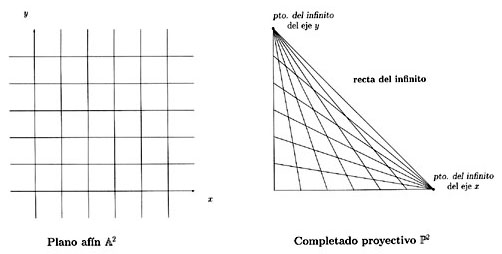
\includegraphics[width=0.5\linewidth]{ppro}
\caption{Plano afín vs Plano proyectivo}
\label{fig:ppro}
\end{figure}

Normalmente cuando hablamos de un plano nos referimos al plano afín, donde dos rectas paralelas lo seguirán siendo siempre. Para representar un punto en el plano afín sólo nos hacen falta dos coordenadas, $(x,y)$. Aquí, las rectas son soluciones a las ecuaciones del tipo $ax+by+c=0$.\\
Las componentes del plano afín pueden ser expresadas como componentes en el plano proyectivo mediante la aplicación $(x,y) \mapsto (x,y,1)$, a estas coordenadas las que llamaremos \textbf{coordenadas homogéneas}. Entonces, hacemos definimos una relación de equivalencia y decimos que el punto $(kx,ky,k)$ es el mismo punto que $(x,y,1)$ en el plano proyectivo. Por tanto, dada una tripleta $(x,y,k), k\neq0$, la llevamos a coordenadas homogéneas dividiendo cada término por $k$. Podríamos decir entonces que el plano afín es un caso concreto del plano proyectivo en el que la recta del infinito tiene un valor prefijado. Una vez descritos los espacios, procedemos a escribir las diferencias a través de las transformaciones afines y proyectivas.\\
Las \textbf{transformaciones afines} son aquellas que mantienen el paralelismo y las proporciones. Son giros, traslaciones, escalados o cizallas. Dejan en el infinito a los puntos del infinito, y no llevan al infinito a los puntos que no están. 
En cambio, las \textbf{transformaciones proyectivas} nos permiten proyectar una imagen plana de manera que resulte real para el ojo humano. Estas transformaciones conservan las intersecciones de rectas, los puntos de tangencia, la concurrencia y la colinearidad.



%----------------------------------------------------------------------------------------
%	Cuestion 2
%----------------------------------------------------------------------------------------

\section{Cuestión 2}

\subsubsection{Enunciado}

Verificar que en coordenadas homogéneas el vector de la recta definida por dos puntos puede calcularse como el producto vectorial de los vectores de los puntos (l = x \textsf{x} x'). De igual modo el punto intersección de dos rectas l y l' está dado por x = l \textsf{x} l'

\subsubsection{Solución}



%----------------------------------------------------------------------------------------
%	Cuestion 3
%----------------------------------------------------------------------------------------

\section{Cuestión 3}

\subsubsection{Enunciado}

Sean x y l un punto y una recta respectivamente en un plano proyectivo P1 y suponemos que la recta l pasa por el punto x, es decir l$^{T}$x=0. Sean x' y l' un punto y una recta del plano proyectivo P' donde al igual que antes l'$^{T}$x'=0.
Supongamos que existe una homografía de puntos H entre ambos planos proyectivos, es decir x'=Hx. Deducir de las ecuaciones anteriores la expresión para la homografía G que relaciona los vectores de las rectas, es decir G tal que l'=Gl. Justificar la respuesta


\subsubsection{Solución}

%----------------------------------------------------------------------------------------
%	Cuestion 4
%----------------------------------------------------------------------------------------

\section{Cuestión 4}

\subsubsection{Enunciado}

Identificar los movimientos elementales (traslación, giro, escala, cizalla, proyectivo) representados por las homografías H1, H2, H3 y H4:

\begin{figure}[H]
\centering
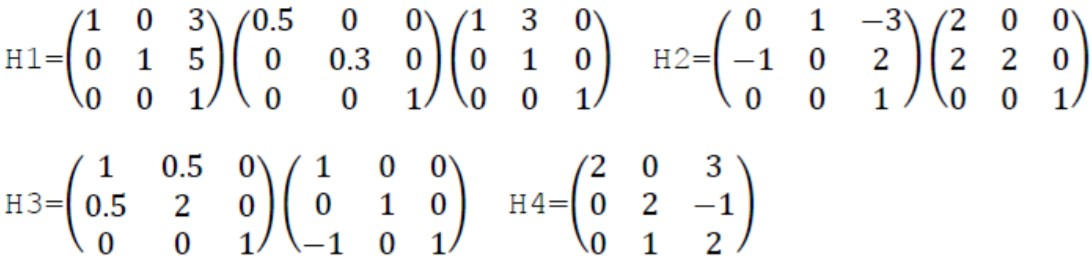
\includegraphics[width=1\linewidth]{Screenshot_1}
\label{fig:screenshot1}
\end{figure}


\subsubsection{Solución}

Para realizar este ejercicio se ha consultado el apartado 2 de \url{http://dip.sun.ac.za/~stefan/TW793/attach/notes/homography_estimation.pdf} en el cual se describen que representa cada uno de los componentes de la matriz de homografía.

La primera matriz $H_1$ es composición de una traslación, un escalado y una cizalla.\\
Las matrices que componen $H_2$ se pueden descomponer a su vez en una traslación compuesta con un giro, y en un escalado compuesto con una cizalla:
\[ H_2 = \left( \begin{array}{lrc}
0 & 1 & -3 \\
-1 & 0 & 2 \\
0 & 0 & 1 \\ \end{array} \right)
\left( \begin{array}{lrc}
2 & 0 & 0 \\
2 & 2 & 0 \\
0 & 0 & 1 \\ \end{array} \right) =\]
\[=  \left( \begin{array}{lrc}
1 & 0 & -3 \\
0 & 1 & 2 \\
0 & 0 & 1 \\ \end{array} \right)
\left( \begin{array}{lrc}
0 & 1 & 0 \\
-1 & 0 & 0 \\
0 & 0 & 1 \\ \end{array} \right)
\left( \begin{array}{lrc}
2 & 0 & 0 \\
0 & 2 & 0 \\
0 & 0 & 1 \\ \end{array} \right)
\left( \begin{array}{lrc}
1 & 0 & 0 \\
1 & 1 & 0 \\
0 & 0 & 1 \\ \end{array} \right)  
\]
Las matrices que componen $H_3$ son una cizalla, un escalado y una proyección:
\[ H_3 = \left( \begin{array}{lrc}
1 & 0.5 & 0 \\
0.5 & 2 & 0 \\
0 & 0 & 1 \\ \end{array} \right)
\left( \begin{array}{lrc}
1 & 0 & 0 \\
0 & 1 & 0 \\
-1 & 0 & 1 \\ \end{array} \right) =\] 
\[=	\left( \begin{array}{lrc}
1 & 0.25 & 0 \\
0.5 & 1 & 0 \\
0 & 0 & 1 \\ \end{array} \right)
\left( \begin{array}{lrc}
1 & 0 & 0 \\
0 & 2 & 0 \\
0 & 0 & 1 \\ \end{array} \right)
\left( \begin{array}{lrc}
1 & 0 & 0 \\
0 & 1 & 0 \\
-1 & 0 & 1 \\ \end{array} \right)\]
Las matrices que componen $H_4$ son una traslación, un escalado, una cizalla y una proyección. La descomposición de ha obtenido calculando inversas:
\[ H_4 = \left( \begin{array}{lrc}
2 & 0 & 3 \\
0 & 2 & -1 \\
0 & 1 & 2 \\ \end{array} \right) =\]
\[=	\left( \begin{array}{lrc}
1 & 0 & 3/2 \\
0 & 1 & -1/2 \\
0 & 0 & 1 \\ \end{array} \right)
\left( \begin{array}{lrc}
2 & 0 & 0 \\
0 & 5/2 & 0 \\
0 & 0 & 1 \\ \end{array} \right)
\left( \begin{array}{lrc}
1 & -3/4 & 0 \\
0 & 1 & 0 \\
0 & 0 & 1 \\ \end{array} \right)
\left( \begin{array}{lrc}
1 & 0 & 0 \\
0 & 1 & 0 \\
0 & 1 & 2 \\ \end{array} \right)\] 

%----------------------------------------------------------------------------------------
%	Cuestion 5
%----------------------------------------------------------------------------------------

\section{Cuestión 5}

\subsubsection{Enunciado}

¿Cuáles son las propiedades necesarias y suficientes para que una matriz defina una homografía entre planos? Justificar la respuesta

\subsubsection{Solución}

La correspondencia lineal: x' = Hx viene definida como:

\begin{figure}[H]
\centering
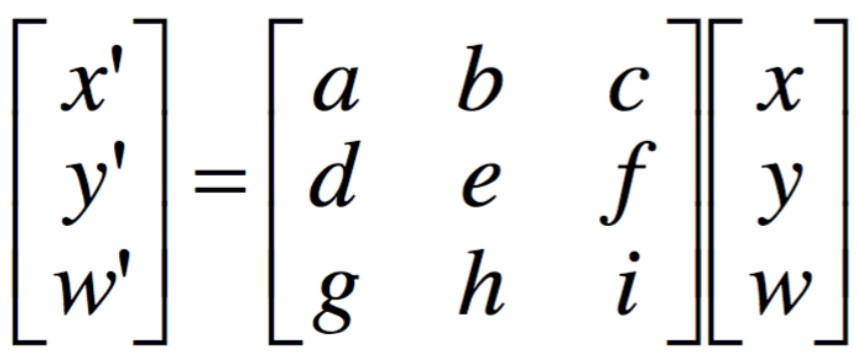
\includegraphics[width=0.7\linewidth]{ej5}
\caption{}
\label{fig:ej5}
\end{figure}

Una de las propiedades que podemos deducir de una homografía H es que debe existir una correspondencia lineal entre los vectores expresados en coordenadas homogéneas de 3 dimensiones. Además el determinante de la matriz H debe ser distinto de 0.
Como H es una matriz no singular (es decir, su determinante nunca es nulo), se podrán invertir las transformaciones proyectivas y la inversa de H será también una proyectividad.
La matriz H se podrá multiplicar por un valor que no sea cero, sin que la transformación proyectiva varíe.

%----------------------------------------------------------------------------------------
%	Cuestion 6
%----------------------------------------------------------------------------------------

\section{Cuestión 6}

\subsubsection{Enunciado}

¿Qué propiedades de la geometría de un plano quedan invariantes si se aplica una homografía general sobre él? Justificar la respuesta.

\subsubsection{Solución}

Las homografías son transformaciones proyectivas que establecen correspondencia entre elementos
iguales, por lo tanto, la homografía conserva la naturaleza de los elementos transformados teniendo unas propiedades invariantes como que un punto se transforma en otro punto, una recta se transforma en otra recta, y un plano se transforma en otro plano. Por lo tanto, la traslación, giro y afinidad serán homografías.
Cuando se aplica una homografía, se conservará la linealidad de la transformación y si dos lineas se cortasen, se conservaría la congruencia/concurrencia.

%----------------------------------------------------------------------------------------
%	Cuestion 7
%----------------------------------------------------------------------------------------

\section{Cuestión 7}

\subsubsection{Enunciado}

¿Cuál es la deformación geométrica más fuerte que se puede producir sobre la imagen de un plano por el punto de vista de la cámara? Justificar la respuesta.

\subsubsection{Solución}

En la deformación proyectiva se conservará de la imagen inicial únicamente los vértices y las líneas rectas, por tanto en la proyectiva no sólo no hay noción de distancia, sino que tampoco hay noción alguna de paralelismo.

%----------------------------------------------------------------------------------------
%	Cuestion 8
%----------------------------------------------------------------------------------------

\section{Cuestión 8}

\subsubsection{Enunciado}

¿Qué información de la imagen usa el detector de Harris para seleccionar puntos? ¿El detector de Harris detecta patrones geométricos o fotométricos? Justificar la contestación.

\subsubsection{Solución}

El detector de Harris usa los cambios de intensidad en dos direcciones (el gradiente) para seleccionar puntos susceptibles a ser esquinas en la imagen. El detector Harris por tanto es capaz de encontrar patrones geométricos ya que los puntos que detecta suelen corresponder con esquinas (que son formas geométricas) y no son simples cambios de intensidad puntuales. También podríamos decir que detecta patrones fotométricos ya que en definitiva la información obtenida es relativa a los cambios de intensidad.

%----------------------------------------------------------------------------------------
%	Cuestion 9
%----------------------------------------------------------------------------------------

\section{Cuestión 9}

\subsubsection{Enunciado}

¿Sería adecuado usar como descriptor de un punto Harris los valores de los píxeles de su región de soporte? En caso positivo identificar cuando y justificar la respuesta 

\subsubsection{Solución}

No sería adecuado ya que al usar los valores de la región de soporte como descriptor haríamos que este fuera demasiado sensible a transformaciones como escalados, rotaciones, cizallas y proyecciones. Es decir, aunque estas transformaciones no afectaran a la detección de la esquina, si afectarían a que el punto Harris detectado se pudiera identificar en la imagen.

%----------------------------------------------------------------------------------------
%	Cuestión 10
%----------------------------------------------------------------------------------------

\section{Cuestión 10}

\subsubsection{Enunciado}

¿Qué información de la imagen se codifica en el descriptor de SIFT? Justificar la contestación. 

\subsubsection{Solución}

Una vez encontrados los KeyPoint, lo que hacemos es calcular los descriptores para cada punto de forma que sea fácil identificarlo y parcialmente invariante a la iluminación, punto de vista…
Los descriptores SIFT son invariantes a cambios afines menores y para probar el carácter distintivo de estos, se iguala la precisión que se mide contra un número variable de puntos clave en la imagen, demostrando que la adecuación de la precisión disminuye los tamaños grandes de imágenes.\\
\\
En definitiva, los descriptores SIFT contienen puntos de interés de las imágenes que serán usados para encontrar coincidencias con otro conjunto de descriptores de otra imagen.

%----------------------------------------------------------------------------------------
%	Cuestion 11
%----------------------------------------------------------------------------------------

\section{Cuestión 11}

\subsubsection{Enunciado}

Describa un par de criterios que sirvan para establecer correspondencias (matching) entre descriptores de regiones extraídos de dos imágenes. Justificar la idoneidad de los mismos 

\subsubsection{Solución}

Una forma para determinar un criterio es el de imponer un umbral de distancia para que, si la distancia entre dos descriptores de dos puntos está por debajo del umbral fijado los marcamos como en correspondencia.

%----------------------------------------------------------------------------------------
%	Cuestion 12
%----------------------------------------------------------------------------------------

\section{Cuestión 12}

\subsubsection{Enunciado}

Cual es el objetivo principal en el uso de la técnica RANSAC. Justificar la respuesta

\subsubsection{Solución}

RANSAC se define como un consenso de muestra aleatoria, el cual tiene 5 pasos a seguir:

\begin{itemize}
	\item Elegir aleatoriamente s muestras (siendo s el tamaño mínimo que permite encajar un modelo)
	\item Colocar un modelo (por ejemplo, una línea) para las muestras
	\item Contar el número de inliers que caben en el modelo aproximadamente
	\item Repetir N veces
	\item Elegir el modelo que tiene el mayor conjunto de inliers.
\end{itemize}

Esta técnica tiene distintos Pros como por ejemplo que es simple, aplicable a muchos problemas diferentes y suele funcionar bien en la práctica. Por otro lado algunos de sus contras serían
el ajuste de parámetros para que de unos buenos resultados y que en ocasiones requiere el uso de muchas iteraciones.\\
\\
En definitiva, el objetivo de RANSAC sería calcular, mediante un método iterativo, los parámetros de un modelo matemático de un conjunto de datos observados que contiene valores atípicos.

%----------------------------------------------------------------------------------------
%	Cuestion 13
%----------------------------------------------------------------------------------------

\section{Cuestión 13}

\subsubsection{Enunciado}

¿Si tengo 4 imágenes de una escena de manera que se solapan la 1-2, 2-3 y 3-4. ¿Cuál es el número mínimo de puntos en correspondencias necesarios para montar un mosaico? Justificar la respuesta 

\subsubsection{Solución}

El mínimo número de puntos para calcular una homografía es 4, por tanto lo ideal sería que los 4 puntos estuvieran en las 4 imágenes y que estos siempre se pusieran en correspondencia. Como sin imágenes distintas que se solapan, el número mínimo de puntos sería 16 ya que contamos que son puntos distintos que se ponen en correspondencia.\\
\\
En este caso solamente tendremos tres homografías que calcular, la de 1-2,2-3 y 3-4, por lo que tendríamos que calcular 4 puntos en la primera imagen que se corresponderán con 4 de la segunda, 3 de los 4 puntos de la segunda imagen más un quinto estarían en correspondencia con 4 de la tercera imagen, y de nuevo 3 de los 4 mas un quinto de la tercera  estarían en correspondencia con 4 puntos de la cuarta imagen. Por lo tanto, en total tendríamos\textbf{ 18 punto}s a calcular.

%----------------------------------------------------------------------------------------
%	Cuestion 14
%----------------------------------------------------------------------------------------

\section{Cuestión 14}

\subsubsection{Enunciado}

En la confección de un mosaico con proyección rectangular es esperable que aparezcan deformaciones de la realidad. ¿Cuáles y porqué?.¿Bajo qué condiciones esas deformaciones podrían desaparecer? Justificar la respuesta 

\subsubsection{Solución}

Es esperable que haya algunas deformaciones debido, por ejemplo, al cambio de punto de vista desde el que se toma la fotografía. Las deformaciones serán más notables si cada imagen del mosaico tiene puntos en común que están alejados unos de otros o el ángulo de visión del mosaico es grande.\\
Otros ejemplos de deformaciones se producen debido a la dificultad para recoger varias imágenes simultáneamente y por tanto pueden cambiar las condiciones de la escena a capturar como la luz o lo que aparezca en el paisaje como por ejemplo las nubes.


\end{document}